\documentclass[english,serif,mathserif,xcolor=pdftex,dvipsnames,table]{beamer}

\usepackage[T1]{fontenc}
\usepackage[utf8]{inputenc}

\usetheme[informal]{s3it}
\usepackage{s3it}

\title[1. Basics]{%
  A Short and Incomplete Introduction to Python
}
\subtitle{\bfseries Part 1: Basic Python syntax}
\author[R.~Murri]{%
  \textbf{Riccardo Murri} \texttt{<riccardo.murri@uzh.ch>}, \\
  Sergio Maffioletti \texttt{<sergio.maffioletti@uzh.ch>}
  \\
  S3IT: Services and Support for Science IT,
  \\
  University of Zurich
}
\date{January 25--26, 2018}


\begin{document}

% title frame
\maketitle

\part{Python basics}

\begin{frame}[fragile]
  \frametitle{Lines of Python code}
  Line of Python code are ended by the ``new line'' character. (I.e., when you
  press the \emph{Enter} key.)

  \+
  A line can be continued onto the next by ending it with the
  character `\texttt{\textbackslash}'; for example:
\begin{semiverbatim}
\In "hello" + \textbackslash
\Ct " world!"
\Out 'hello world!'
\end{semiverbatim}
  The prompt changes to `\texttt{...}' on continuation lines.

  \+\scriptsize
  Reference:
  \url{http://docs.python.org/reference/lexical_analysis.html#line-structure}
\end{frame}


\section{Variables, data types, and operations}

\begin{frame}[fragile]
  \frametitle{String literals, I}
  There are several ways to express string literals in Python.

  \+
  Single and double quotes can be used interchangeably:
\begin{semiverbatim}
\In "a string" == 'a string'
\Out True
\end{semiverbatim}

  \+
  You can use the single quotes inside double-quoted strings, and viceversa:
\begin{semiverbatim}
\In a = "Isn't it ok?"
\In b = '"Yes", he said.'
\end{semiverbatim}
\end{frame}


\begin{frame}[fragile]
  \frametitle{String literals, II}
  Multi-line strings are delimited by three quote characters.
\begin{lstlisting}[showstringspaces=false]
~\In~ a = """This is a string,
~\Ct~ that extends over more
~\Ct~ than one line.
~\Ct~ """
\end{lstlisting}

  \+ In other words, you need not use the backslashes
  ``\texttt{\textbackslash}'' at the end of the lines.
\end{frame}


\begin{frame}[fragile]
  \frametitle{Operators}
  All the usual unary and binary arithmetic operators are
  defined in Python: \texttt{+}, \texttt{-}, \texttt{*}, \texttt{/},
  \texttt{**}~(exponentiation), \texttt{<{}<}, \texttt{>{}>}, etc.

  \+
  Logical operators are expressed using plain English words:
  \texttt{and}, \texttt{or}, \texttt{not}.

  \+
  Numerical and string comparison also follows the usual notation:
  \texttt{<}, \texttt{>}, \texttt{<=}, \texttt{==}, \texttt{!=},
  \ldots

  \+
  \begin{references}
    \tiny
    \begin{itemize}
    \item
      \url{http://docs.python.org/library/stdtypes.html#boolean-operations-and-or-not}
    \item
      \url{http://docs.python.org/library/stdtypes.html#comparisons}
    \end{itemize}
  \end{references}
\end{frame}


\begin{frame}
  \frametitle{Your first exercise}
  %\href{http://www.pythonchallenge.com}{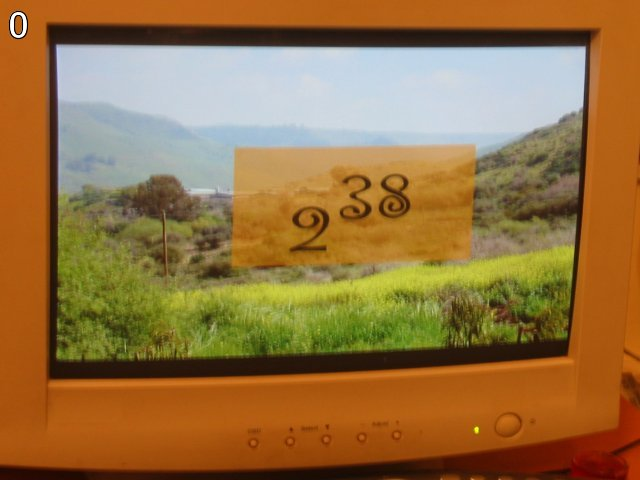
\includegraphics[width=\linewidth]{fig/2to38}}
    \begin{center}
      {\Large How much is \href{http://www.pythonchallenge.com}{$2^{144}$} ?}

      \+ (You have 1 minute time.)
    \end{center}
\end{frame}


\begin{frame}[fragile]
  \frametitle{Operators, II}
  \smaller

  Some operators are defined for non-numeric types:
\begin{lstlisting}
>>> "Py" + 'thon'
'Python'
\end{lstlisting}

  \+
  Some support operands of mixed type:
\begin{lstlisting}
>>> "a" * 2
'aa'
>>> 2 * "a"
'aa'
\end{lstlisting}

  \+
  Some do not:
\begin{lstlisting}[basicstyle=\footnotesize\ttfamily]
>>> "aaa" / 3
Traceback (most recent call last):
  File "<stdin>", line 1, in <module>
TypeError: unsupported operand type(s) for /: 'str' and 'int'
\end{lstlisting}
\end{frame}


\begin{frame}[fragile]
  \frametitle{Operators, III}
  The ``\texttt{\%}'' operator computes the remainder of integer division.
\begin{semiverbatim}
\In 9 % 2
\Out 1
\end{semiverbatim}

  \+ It also doubles up as \emph{string interpolation operator}, but the
  `\lstinline|format()|' method (see next slide) is more convenient.
\end{frame}


\begin{frame}[fragile]
  \frametitle{String interpolation}
  The \lstinline|.format()| method can be used to substitute values into placeholder
  strings.

  \+ \pause
  Placeholders can indicate substitutions by ordinal number:
\begin{lstlisting}[basicstyle=\footnotesize\ttfamily]
>>> "This is slide ~\alt<2>{\HL{\small\ttfamily\{0\}}}{\small\ttfamily\{0\}}~ of ~\alt<2>{\HL{\small\ttfamily\{1\}}}{\small\ttfamily\{1\}}~".format(20, 1001)
'This is slide 20 of 1001.'
\end{lstlisting}

  \+ \pause
  You can use names instead of numbers (then the order parameter occur in
  \lstinline|format()| does not matter):
\begin{lstlisting}[basicstyle=\footnotesize\ttfamily]
>>> "Today is ~\alt<3>{\HL{\small\ttfamily\{month\}}}{\{month\}}~ ~\alt<3>{\HL{\small\ttfamily\{day\}}}{\small\ttfamily\{day\}}~".format(day=2, month='March')
'Today is March 2'
\end{lstlisting}

  \begin{references}
    \url{https://pyformat.info/}
  \end{references}
\end{frame}


\begin{frame}[fragile]
  \frametitle{Assignment, I}
  Assignment is done via the `\texttt{=}' statement:
\begin{semiverbatim}
\In a = 1
\In print(a)
\Out 1
\end{semiverbatim}

  \+
  There are a few shortcut notations:
  \begin{itemize}
  \item[] \texttt{\emph{a} += \emph{b}} is short for \texttt{\emph{a} = \emph{a} + \emph{b}},
  \item[] \texttt{\emph{a} -= \emph{b}} is short for \texttt{\emph{a} = \emph{a} - \emph{b}},
  \item[] \texttt{\emph{a} *= \emph{b}} is short for \texttt{\emph{a} = \emph{a} * \emph{b}},
  \item[]   etc. --- one for every legal operator.
  \end{itemize}
\end{frame}


\begin{frame}[fragile]
  \frametitle{Assignment, II}

  \textbf{Python variables are just ``names'' given to values.}

  \+
  This allows you to \emph{reference} the string \texttt{'Python'}
  by the \emph{name} \texttt{a}.  But also by another name \texttt{b}:

  \+
  \includegraphics[width=1.00\linewidth]{fig/a=b.pdf}

  \+
  The \emph{same} object can be given many names!

  \+
  \begin{seealso}
    \scriptsize \url{http://excess.org/article/2014/04/bar-foo/}
  \end{seealso}
\end{frame}


\begin{frame}[fragile]
  \frametitle{The \texttt{is} operator}

  The \texttt{is} operator allows you to test whether two names refer
  to the same object:
\begin{lstlisting}
>>> a = 1
>>> b = 1
>>> a is b
True
\end{lstlisting}

\end{frame}


\begin{frame}[fragile]
  \frametitle{Basic types}
  Basic object types in Python 3:
  \begin{description}
  \item[bool] The class of the two boolean constants \texttt{True}, \texttt{False}.
  \item[int] Integer numbers: \texttt{1}, \texttt{-2}, \ldots
  %   up to \texttt{9223372036854775807} (on a 64-bit machine)
  % \item[long] Integer numbers of arbitrary size; Python switches
  %   automatically from \texttt{int} to \texttt{long} when needed.
  \item[float] Double precision floating-point numbers, e.g.:
    \texttt{3.1415}, \texttt{-1e-3}.
  \item[bytes] String of byte-size characters.
  \item[str] Text (string of UNICODE characters).
  %\item[unicode] Strings of UNICODE characters.
  \item[list] Mutable list of Python objects
  \item[dict] Key/value mapping
  \end{description}

  \+ The type of a Python object can be gotten via the \texttt{type()} function:
\begin{semiverbatim}
{\color{blue}\bfseries In [3]:} type('hello')
{\color{red}\bfseries Out[3]:} str
\end{semiverbatim}
\end{frame}


\part{Appendix}

\section{Caveats}

\begin{frame}[fragile]
  \frametitle{All variables are references}

  In Python, \textbf{all objects are ever passed by reference}.

  \+
  In particular, \textbf{variables always store a reference to an
    object}, never a copy!

  \+
  Hence, you have to be careful when modifying objects:
\begin{lstlisting}
>>> a = [1,2,3]
>>> b = a
>>> b.remove(2)
>>> print(a)
\end{lstlisting}
  \only<1>{%
\vspace{-1.5em}
\begin{semiverbatim}
\emph{???}
\end{semiverbatim}
    \begin{center}
      \textbf{Q}: How many items are in the \texttt{a} list now?
    \end{center}
  }%
  \only<2>{%
\vspace{-1.5em}
\begin{semiverbatim}
[1, 3]
\end{semiverbatim}

   \+
   \href{http://tinyurl.com/cq3tcab}{Run this example} in the
   \href{http://pythontutor.com/}{Online Python Tutor} to better
   understand what's going on.

   \+
   {\small \em
     This applies particularly for variables that capture the arguments
     to a function call!}
}%
\end{frame}


\begin{frame}[fragile]
  \frametitle{All variables are references (demo)}

  \href{http://www.pythontutor.com/}{www.pythontutor.com}
  \+

  \only<1>{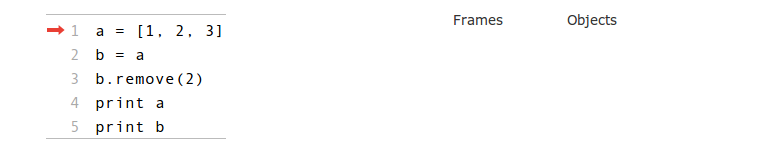
\includegraphics[width=1.2\textheight]{fig/t1_screenshot_1.png}}
  \only<2>{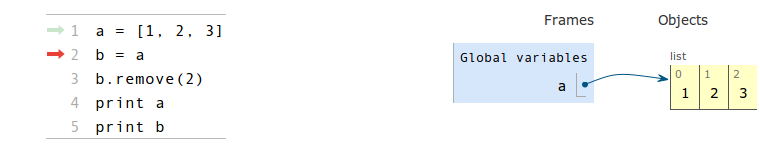
\includegraphics[width=1.2\textheight]{fig/t1_screenshot_2.png}}
  \only<3>{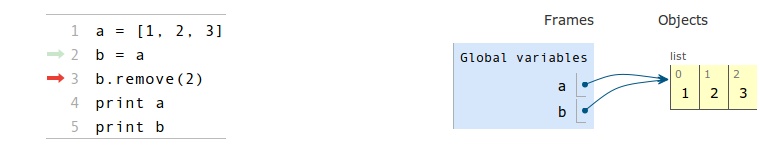
\includegraphics[width=1.2\textheight]{fig/t1_screenshot_3.png}}
  \only<4>{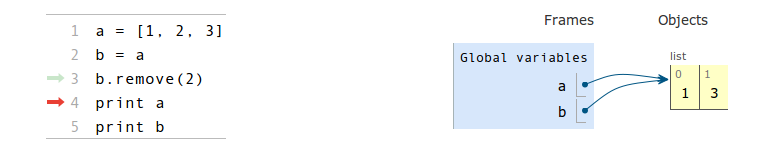
\includegraphics[width=1.2\textheight]{fig/t1_screenshot_4.png}}

\end{frame}



\end{document}

%%% Local Variables:
%%% mode: latex
%%% TeX-master: t
%%% End:
